% Настройки документа
\documentclass[a4paper, 11pt]{article}


\usepackage{amsmath}
\usepackage{amssymb}
\usepackage{hyperref}
\usepackage{url}
\usepackage{a4wide}
\usepackage[utf8]{inputenc}
\usepackage[main = russian, english]{babel}
\usepackage[pdftex]{graphicx}
\usepackage{float}
\usepackage{subcaption}
\usepackage{indentfirst} 


\newenvironment{compactlist}{
	\begin{list}{{$\bullet$}}{
			\setlength\partopsep{0pt}
			\setlength\parskip{0pt}
			\setlength\parsep{0pt}
			\setlength\topsep{0pt}
			\setlength\itemsep{0pt}
		}
	}{
	\end{list}
}

\newcommand{\myint}[4]{\int\limits_{#1}^{#2}#3\,d#4}

\DeclareMathOperator{\sgn}{sgn}


% Документ
\begin{document}


% Титульная страница
\thispagestyle{empty}
\begin{center}
\ \vspace{-3cm}


\includegraphics[width=0.5\textwidth]{img/msu.eps}\\

{\scshape Московский государственный университет имени М.~В.~Ломоносова}\\
Факультет вычислительной математики и кибернетики\\
Кафедра системного анализа

\vfill

{\LARGE Отчёт по практикуму}

\vspace{1cm}

{\Huge\bfseries <<Быстрое преобразование Фурье>>}
\end{center}
\vspace{3cm}
\begin{flushright}
  \large
  \textit{Студент 315 группы}\\
  К.\,Ю.~Егоров

  \vspace{5mm}

  \textit{Руководитель практикума}\\
  к.ф.-м.н., доцент И.\,В.~Рублёв
\end{flushright}
\vfill
\begin{center}
Москва, 2018
\end{center}
\clearpage


% Страница с оглавлением
\tableofcontents
\clearpage

\clearpage
% Постановка задачи
\section{Постановка задачи}

    \subsection{Общая формулировка задачи}
        
        Дана система функций
        \begin{equation} \label{eq:system}
            \begin{cases} 
                f_1 = \frac{1 - \cos^2t}{t},   \\ \\
                f_2 = t \cdot e^{-2t^2},      \\ \\
                f_3 = \frac{2}{1+3t^6},       \\ \\
                f_4 = e^{-5|t|}\cdot \ln(3+t^4). 
            \end{cases}
        \end{equation}
        
        Для каждой функции из системы~\eqref{eq:system} требуется:
        \begin{enumerate}
            \item Получить аппроксимацию преобразования Фурье~$F(\lambda)$ при помощи быстрого преобразования Фурье, выбирая различный шаг дискретизации и различные окна, ограничивающие область определения функции~$f(t)$.
            \item Построить графики получившихся аппроксимаций $F(\lambda)$.
            \item Для функций $f_1(t)$ и $f_2(t)$ из системы~\eqref{eq:system} вычислить аналитически преобразование Фурье~$F_1(\lambda)$ и $F_2(\lambda)$ и сравнить графики, полученные в результате аналитического решения и аппроксимации с помощью быстрого преобразования Фурье.
            \item Проиллюстрировать на графиках эффекты ряби и наложения хвостов. Продемонстрировать причины возникновения этих эффектов и возможные способы их устранения.
        \end{enumerate}
        
    \subsection{Формальная формулировка задачи}
        Для решения поставленной задачи необходимо реализовать на языке~\textit{MATLAB} функцию~\texttt{plotFT}, принимающую следующие аргументы:
        \begin{itemize}
            \item \texttt{hFigure} --- указатель на фигуру, в которой требуется отобразить графики.
            \item \texttt{fHandle} --- указатель на функцию (\textit{function handle}), аппроксимацию которой необходимо получить.
            \item \texttt{fFTHandle} --- указатель на функцию (\textit{function handle}), являющейся преобразованием Фурье функции, переданной как \texttt{fHandle}, либо пустой вектор.
            \item \texttt{step} --- положительное число, задающее шаг дискретизации $\Delta t$.
            \item \texttt{inpLimVec} --- вектор-строка, задающая окно $[a, b]$ для функции, переданной как \texttt{fHandle}. Первый элемент вектора содержит $a$, второй --- $b$, причем $a < b$, но не обязательно $a = -b$.
            \item \texttt{outLimVec} --- вектор-строка, задающая окно $[c, d]$ для построения графика преобразования Фурье и его аппроксимации. Необязательный параметр. В случае, если параметр не задан, следует использовать установленные в фигуре \texttt{hFigure} пределы или определить свои разумным способом.
        \end{itemize}
        
        Данная функция должна строить графики вещественной и мнимой частей численной аппроксимации преобразования Фурье функции, переданной как \texttt{fHandle} и, если задан \texttt{fFTHandle}, --- графики соответствующих частей полученного аналитически преобразования Фурье, передаваемого как \texttt{fFTHandle}. 
        Кроме того, функция должна возвращать структуру, содержащую следующие параметры:
        \begin{itemize}
            \item \texttt{nPoints} --- число вычисляемых узлов сеточной функции, рассчитываемое по формуле
                $$
                    nPoints = \left \lfloor \frac{b- a}{step} \right \rfloor.        
                $$
            \item \texttt{step} --- исправленное значение шага дискретизации $\Delta t$, рассчитываемое по формуле
                $$
                    step = \frac{b-a}{nPoints}.
                $$
            \
item \texttt{inpLimVec} --- окно $[a, b]$ для функции, передаваемой как \texttt{fHandle}.
            \item \texttt{outLimVec} --- окно для вывода графика аппроксимации преобразования Фурье функции, передаваемой как \texttt{fHandle}.
        \end{itemize}          
        
        При помощи функции \texttt{plotFT} выполнить общую задачу.

\clearpage
% Аналитическое решение
\section{Аналитическое вычисление преобразований Фурье}
    \subsection{Краткая теоритическая справка} 
        Преобразование Фурье $F(\lambda)$ для функции $f(t)$ задается формулой
        \begin{equation} \label{eq:fourier}
            F(\lambda) = \myint{-\infty}{\infty}{f(t)\cdot e^{-i\lambda t}}{t}.
        \end{equation}       
        
        Для аналитического вычисления преобразования Фурье нам потребуются знания некоторых значений часто встречающихся интегралов.
        
        \textbf{Интеграл Дирихле}
        \begin{equation} \label{eq:Dirichlet_integral}
            \myint{0}{+\infty}{\frac{\sin \: x}{x}}{x} = \frac{\pi}{2}
        \end{equation}
        
        \textbf{Интеграл Пуассона}
        \begin{equation} \label{eq:puasson}
        \myint{0}{+\infty}{e^{-x^2}}{x} = \frac{\sqrt{\pi}}{2}
        \end{equation}
             
        

    \subsection{Вычисление преобразования Фурье первой функции}
        Преобразуем заданную функцию к более удобному виду
        $$
            f_1(t) = \frac{1-\cos^2t}{t} = \frac{\sin^2t}{t} = \frac{1 - \cos2t}{2t}.
        $$
        
        Преобразование Фурье $F_1(\lambda)$ функции $f_1(t)$ по определению~\eqref{eq:fourier} задаётся формулой
        $$
            F_1(\lambda) = \myint{-\infty}{+\infty}{\frac{1 - \cos2t}{2t}\cdot e^{-i\lambda t}}{t}. 
        $$
        
        Вычислим данный интеграл. Распишем $e^{-i\lambda t} = \cos(\lambda t) - i \sin(\lambda t)$ и воспользуемся линейностью интеграла
        $$    
        \myint{-\infty}{+\infty}{\frac{1 - \cos2t}{2t}\cdot e^{-i\lambda t}}{t} = \myint{-\infty}{+\infty}{\frac{1 - \cos2t}{2t}\cdot \cos(\lambda t)}{t} - i\myint{-\infty}{+\infty}{\frac{1 - \cos2t}{2t}\cdot \sin(\lambda t)}{t} =
        $$
        $$
            = \frac{1}{2}\myint{-\infty}{+\infty}{\frac{\cos(\lambda t)}{t}}{t}-\frac{1}{2}\myint{-\infty}{+\infty}{\frac{\cos(2t) \cdot \cos(\lambda t)}{t}}{t}- \frac{i}{2}\myint{-\infty}{+\infty}{\frac{\sin(\lambda t)}{t}} {t} +\frac{i}{2}\myint{-\infty}{+\infty}{\frac{\cos(2t)\cdot \sin(\lambda t)}{t}} {t} = 
        $$
        $$
            = \frac{1}{2}I_1 - \frac{1}{2}I_2 - \frac{i}{2}I_3 + \frac{i}{2}I_4.
        $$
        \begin{enumerate}
            \item Интеграл $I_1$ равен нулю в силу нечётности подынтегральной функции.
            \item Вычислим интеграл $I_2$.
                Воспользуемся формулой тригонометрии
                $$
                    \cos(2t) \cdot \cos(\lambda t) = \frac{\cos((2+\lambda)t) + \cos((2-\lambda)t)}{2}.
                $$
                Тогда, пользуясь линейностью интеграла,
                $$
                    I_2 = \myint{-\infty}{+\infty}{\frac{\cos(2t) \cdot \cos(\lambda t)}{t}}{t} =
                $$
                $$
                    = \frac{1}{2}\myint{-\infty}{+\infty}{\frac{\cos((2+\lambda)t)}{t}} {t}+\frac{1}{2}\myint{-\infty}{+\infty}{\frac{\cos((2-\lambda)t)}{t}} {t}.
                $$
                Каждый из получившихся интегралов после замены переменной сводится к $I_1$. Значит, $I_2$ также равен нулю.
            \item Вычислим интеграл $I_3$. Рассмотрим случаи:
                \begin{enumerate}
                    \item $\lambda = 0$. Интеграл, очевидно, равен нулю.
                    \item $\lambda \neq 0$. Интеграл заменой переменной сводится к интегралу Дирихле~\eqref{eq:Dirichlet_integral}. $$I_2 = \pi \cdot \sgn{\lambda}$$.
                \end{enumerate}
            \item Вычислим интеграл $I_4$. Воспользуемся тригонометрической формулой
                $$
                    \cos(2t)\cdot \sin(\lambda t) = \frac{\sin((\lambda+2)t) + \sin((\lambda-2)t)}{2}.
                $$
                Пользуясь линейностью интеграла и четностью подынтегральных функций получаем
                $$
                    I_4 = \myint{-\infty}{+\infty}{\frac{\cos(2t)\cdot \sin(\lambda t)}{t}} {t} =
                $$
                $$
                    = \myint{0}{+\infty}{\frac{\sin((\lambda+2)t)}{t}} {t} + \myint{0}{+\infty}{\frac{\sin((\lambda-2)t)}{t}} {t}.
                $$
                Рассмотрим случаи:
                    \begin{enumerate}
                        \item $\lambda > 2$. Делая замену переменной, получим интегралы Дирихле~\eqref{eq:Dirichlet_integral}. $$I_4 = \pi$$
                        \item $\lambda = 2$. Второй интеграл обнулится, а первый сводится к интегралу Дирихле~\eqref{eq:Dirichlet_integral}. $$I_4 = \frac{\pi}{2}$$
                        \item $-2 < \lambda < 2 $. Очевидно, что $$I_4 = 0$$.
                        \item $\lambda = -2$. Первый интеграл обнулится, а второй сводится к интегралу Дирихле~\eqref{eq:Dirichlet_integral}. $$I_4 = -\frac{\pi}{2}$$
                        \item $\lambda < -2$. Делая замену переменной, получим интегралы Дирихле~\eqref{eq:Dirichlet_integral}. $$I_4 = -\pi$$
                    \end{enumerate}
        \end{enumerate}
        
        В итоге получаем преобразование Фурье для первой функции
        \begin{equation}
            F(\lambda) = 
            \begin{cases}
                0,                 & \lambda \in (-\infty ; 2)\cup \{ 0 \} \cup (2 ; +\infty) \\
                -\frac{\pi i}{2},  & \lambda \in (0 ; 2)\\
                \frac{\pi i}{2},   & \lambda \in (-2; 2) \\
                \frac{\pi i}{4},   & \lambda = -2 \\
                -\frac{\pi i}{4},  & \lambda = 2 \\
            \end{cases}
        \end{equation}
    
    \subsection{Вычисление преобразования Фурье второй функции}
        Преобразование Фурье $F_2(\lambda)$ функции $f_2(t) = t \cdot e^{-2t^2}$ задаётся формулой
        $$
            F_2(\lambda) = \myint{-\infty}{+\infty}{t \cdot e^{-2t^2} \cdot e^{-i\lambda  t}}{t}.
        $$
        
        Проиллюстрируем цепочку преобразований: 
        $$
            \myint{-\infty}{+\infty}{t \cdot e^{-2t^2} \cdot e^{-i\lambda  t}}{t} = \myint{-\infty}{+\infty}{t \cdot e^{-2t^2-i\lambda  t}}{t} =\myint{-\infty}{+\infty}{t \cdot e^{-\left(2t^2+i\lambda t+\frac{i^2\lambda^2}{8}\right)+\frac{i^2\lambda^2}{8}}}{t} = 
        $$
        $$
            = e^{-\frac{\lambda^2}{8}}\myint{-\infty}{+\infty}{t \cdot e^{-\left( \sqrt{2}t+\frac{i\lambda}{2\sqrt{2}}\right)^2}}{t}=\left[\sqrt{2}t+\frac{i\lambda}{2\sqrt{2}}=s\right]=
        $$
        $$
            =\frac{1}{\sqrt{2}}e^{-\frac{\lambda^2}{8}}\myint{-\infty}{+\infty}{\left(\frac{s}{\sqrt{2}}-\frac{i\lambda}{4}\right)e^{-s^2}}{s}=\frac{1}{4}e^{-\frac{\lambda^2}{8}}\myint{-\infty}{+\infty}{se^{-s^2}}{s} - \frac{i\lambda}{4\sqrt{2}}e^{-\frac{\lambda^2}{8}}\myint{-\infty}{+\infty}{e^{-s^2}}{s}=
        $$
        $$
            \frac{1}{4}e^{-\frac{\lambda^2}{8}}\myint{-\infty}{+\infty}{e^{-s^2}}{s^2} - \frac{i\lambda}{4\sqrt{2}}e^{-\frac{\lambda^2}{8}}\myint{-\infty}{+\infty}{e^{-s^2}}{s}.
        $$
        
        Таким образом, первый интеграл обнуляется, а второй является интегралом Пуассона~\eqref{eq:puasson}. В итоге получаем
        $$
            F_2(\lambda) = -\frac{i \sqrt{\pi}}{4\sqrt{2}} \cdot \lambda \cdot e^{-\frac{\lambda^2}{8}}.
        $$

\clearpage
\section{Описание работы программы}
    \begin{enumerate}
        \item
            Число \texttt{nPoints} отвечает за количество узлов сетки и вычисляется следующим образом
            $$
                nPoints = \left \lfloor \frac{b-a}{step} \right \rfloor.        
            $$
            Оно необходимо нам для задания дискретизации функции.
        \item
            Вычисляем новое значение шага по формуле
            $$
                \Delta t = \frac{b-a}{nPoints}.
            $$
        \item
            Тогда периодом будет
            $$
                T = \frac{2\pi}{\Delta t}.            
            $$
            Следовательно преобразование Фурье будем вычислять на отрезке $\left[ -\frac{\pi}{\Delta t}; \frac{\pi}{\Delta t} \right]$.
        \item
            Для того, чтобы получить преобразование Фурье, необходимо воспользоваться следующими функциями из \texttt{MATLAB}:
            \begin{enumerate}
                \item
                    Функция \texttt{fft} принимает вектор значений исходной функции $f(t)$ и возвращает вектор дискретного преобразования Фурье $\widetilde{\widetilde{F}}(\lambda)$, симметрично отражённый относительно нашей функции $f(t)$.
                \item
                    Функция \texttt{fftshift} принимает вектор $\widetilde{\widetilde{F}}(\lambda)$, делит его на две равные части и переставляет эти части между собой. Если выполнить функции последовательно, то получим $F_{discr.}(n)$ --- дискретное преобразование Фурье. Для получения аппроксимации непрерывного преобразования Фурье необходимо вектор дискретного преобразования Фурье домножить на шаг дискретизации. Ниже преведено краткое обоснование этого факта.%Стоит отметить, что полученное при помощи функции \texttt{fft} преобразование $\widetilde{F}(\lambda)$ определено периодически на $\left[ 0,\; \frac{2\pi}{\Delta t} \right]$, а искомое нами преобразование Фурье --- на $\left[ -\frac{\pi}{\Delta t}, \; \frac{\pi}{\Delta t} \right]$. При этом значения этих преобразований совпадают с точностью до сдвига на полупериод.
            \end{enumerate}
	        Преобразование Фурье дискретизированной и периодически продолженной функции $f(t)$ имеет вид
            $$
                (f(\cdot)\cdot d_{\Delta t}(\cdot)\cdot h_{\Delta_0}(\cdot) * d_{\Delta_0})(t) \longleftrightarrow \frac{2\pi}{\Delta_0 \Delta t}(\widetilde{F}(\cdot) * d_{\frac{2\pi}{\Delta_0}}(\cdot))(\lambda).
            $$
            Это преобразование с точностью до ряби и наложения спектра совпадает с преобразованием Фурье функции $f(t)$, то есть
            $$
                F(\lambda_n) \approx \frac{2\pi}{\Delta_0\Delta t} \widetilde{F}(\lambda_n),
            $$
            где $\lambda_n = \frac{2\pi n}{\Delta_0},\; n = \overline{0, N-1}$.

            Тогда
            $$
                \widetilde{F}(\lambda_n) = \widetilde{F_n} = \Delta t \cdot F_{discr.}(n).
            $$
        \item
            Наконец, чтобы сместить отрезок в начало координат, домножим наше преобразование Фурье на $e^{-i\lambda \alpha}$, где $\alpha$ --- это точка, которую мы сдвигаем в начало координат. Это можно сделать в силу преобразования
            $$
                f(t-\alpha) \longleftrightarrow e^{-i\lambda\alpha} \cdot F(\lambda).            
            $$
            Сдвиг необходим из-за ограничения на левую границу дискретного преобразования Фурье:
            $$
                f(t) = 0,\; t < 0.            
            $$
    \end{enumerate}
\clearpage
\section{Иллюстрация работы программы}
    \subsection{Первая функция}
    Рассмотрим функцию
    $$
        f_1(t) = \frac{1 - \cos^2t}{t}.    
    $$
    
    Данная функция имеет разрыв первого рода в точке $t = 0$. Исходя из аналитического представления преобразования Фурье $F_1(\lambda)$, мы знаем, что у него есть три точки разрыва ($\lambda = \pm 2; \; 0 )$.
    
    Рассмотрим графики аппроксимации преобразования Фурье для этой функции, выбирая различные шаги дискретизации $\Delta t$, окна, ограничивающего область определения функции $[a;\; b]$, окна вывода преобразования $[c;\; d]$, и сделаем выводы.
    
    \begin{enumerate}
        \item
            $\Delta t = 10^{-4}$, $[a;\; b] = [-50;\; 50]$, $[c;\;d] = [-3;\;3]$.
            
            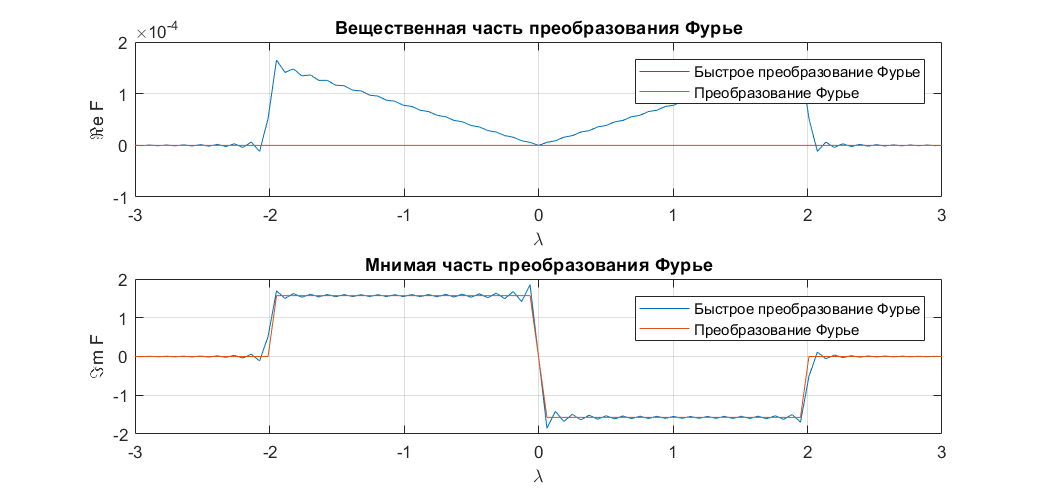
\includegraphics[width=\linewidth]{img/1.png}
            
            \begin{enumerate}
                \item
                    Мнимые части преобразования Фурье, полученные аналитически и численно, совпадают с точностью до ряби, называемой рябью Гиббса. Эта рябь неизбежно возникает в точках разрыва. От этой ряби не возможно избавиться при изменении параметров, но размер ряби пропорционален величине разрыва
			        $$
			        	F(\lambda_0^+) - F(\lambda_0^-) = a,
			        $$
где $\lambda_0$ --- точка разрыва преобразования Фурье $F(\lambda)$.

		            Рассмотрим функцию на отдалении от точки разрыва
                    $$
                        F(\lambda) = F_c(\lambda) + \chi(\lambda - \lambda_0)\left[ F(\lambda_0^+) - F(\lambda_0^-)\right] = F_c(\lambda) + a \chi (\lambda - \lambda_0),
                    $$
                    где $F_c(\lambda)$ --- непрерывная часть преобразования Фурье.

                    Тогда у отклонения есть конечный предсказуемый предел, меньший, чем $\frac{a\rho_1}{\pi} \approx 0,0894\:a$. Эта особенность позволяет сглаживать рябь даже на небольшом отклонении от точек разрыва с помощью специальных фильтров.
                \item
                     Из аналитического представления $F_1(\lambda)$ следует, что вещественная часть аналитического преобразования Фурье равна нулю, в то время, как вещественная часть, полученная численно, по модулю отлична от нуля. Но это отличие сопоставимо с шагом дискретизации. Отметим, что точки разрыва в вещественной и мнимой частях численного преобразования Фурье совпадают. 
            \end{enumerate}
        \item
              $\Delta t = 10^{-4}$, $[a;\; b] = [-400;\; 400]$, $[c;\;d] = [-3;\;3]$.             
              
              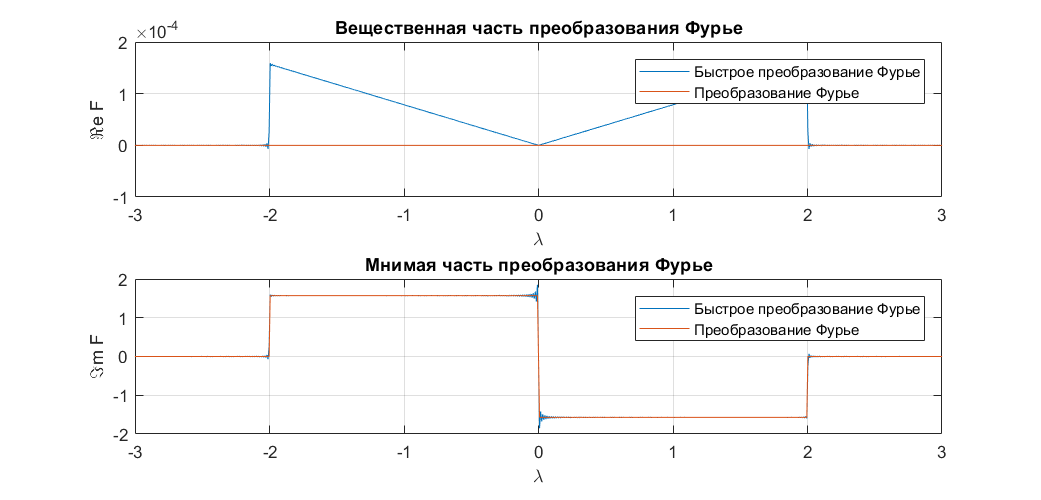
\includegraphics[width=\linewidth]{img/2.png}
              \begin{enumerate}
                  \item
                      Мнимые части преобразования Фурье, полученные численно и аналитически, совпадают с точностью до ряби в точках разрыва. Это связано с тем, что мы увеличили размер окна в 8 раз. Следовательно увеличивая диапозон окна, можно добиться исчезновения ряби Гиббса в точках непрерывности функции $F_1(\lambda)$.
                  \item
                      Ситуация с действительной частью обстоит также, как и в предыдущем пункте.
              \end{enumerate}
        \item
            $\Delta t = 10^{-4}$, $[a;\; b] = [-100;\; 200]$, $[c;\;d] = [-3;\;3]$.             
            
            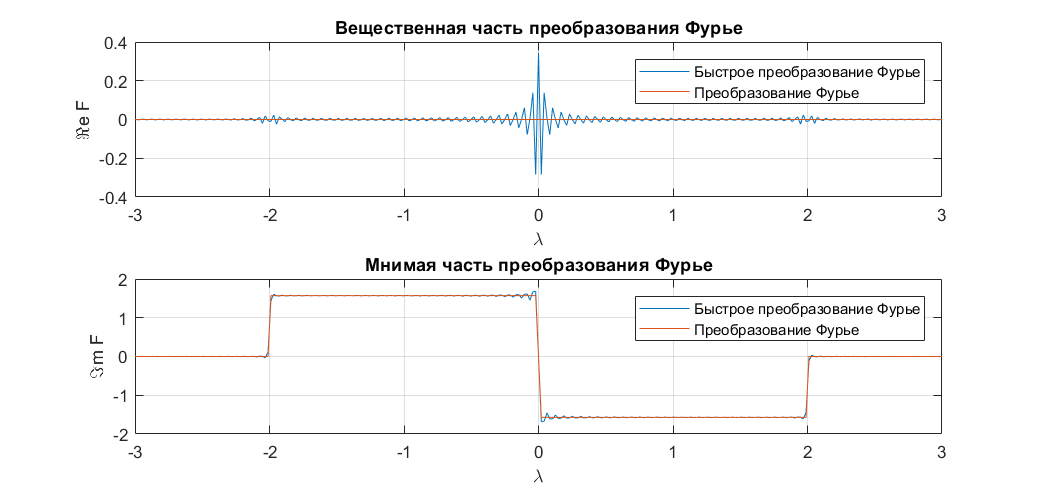
\includegraphics[width=\linewidth]{img/3.png}
            
            \begin{enumerate}
                \item
                     В отличии от предыдущего пункта, здесь мы сместили оконную функцию на 50 единиц вправо, относительно начала координат. На графике вещественной части численного преобразования Фурье видно, что в точках разрыва образовались “пики”. Это явление вызвано свдигом оконной функции. Чем более несимметрично --- тем больше рябь. В то время как рябь в точках непрерывности преобразования Фурье $F(\lambda)$ стремится к нулю при увеличении частоты дискретизации, то уменьшить рябь в точках разрыва можно только сдвигом заданного окна. На несимметричном окне рябь распространяется и на действительную часть графика, где разрыва не наблюдалось. Эту особенность можно проследить из интеграла ошибки $I$, который показывает погрешность по действительной и мнимой части преобразования.
                    $$
                        I = \myint{-\infty}{+\infty}{\left( F(\lambda - \mu) e^{-i\mu t_0} - F(\lambda)e^{-i\mu t_0}\right) \cdot \frac{\sin{\frac{\Delta_0\mu}{2}}}{\lambda\mu}}{\mu},
                    $$
                    где $t_0$ --- сдвиг окна относительно нуля, $\Delta_0$ --- размер окна.
            \end{enumerate}
    \end{enumerate}
    
    \subsection{Вторая функция}
        Рассмотрим функцию
        $$
            f_2(t) = t \cdot e^{-2t^2}.        
        $$  
        
        Как можно видеть, эта функция и её аналитическое преобразование Фурье непрерывны.
        \begin{enumerate}
            \item
                $\Delta t = 10^{-4}$, $[a;\; b] = [-50;\; 50]$, $[c;\;d] = [-10;\;10]$.
                
                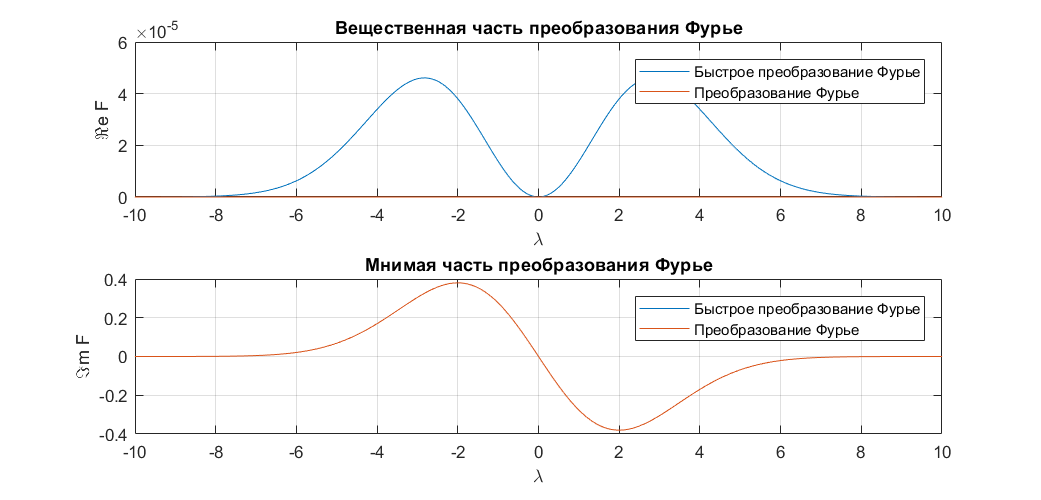
\includegraphics[width=\linewidth]{img/4.png}
                
                \begin{enumerate}
                    \item
                        Мнимые части преобразования Фурье, полученные численно и аналитически, совпадают. 
                    \item
                        Вещественная часть преобразования Фурье, полученная аналитически, равна нулю.А вещественная часть преобразования Фурье, полученная численно, по модулю сопоставима с шагом дискретизации $\Delta t$.
                    \item
                        Отсутствует рябь, ввиду того, что нет точек разрыва.
                \end{enumerate}
            
            \item
                $\Delta t = 10^{-4}$, $[a;\; b] = [-50;\; 300]$, $[c;\;d] = [-10;\;10]$.
                
                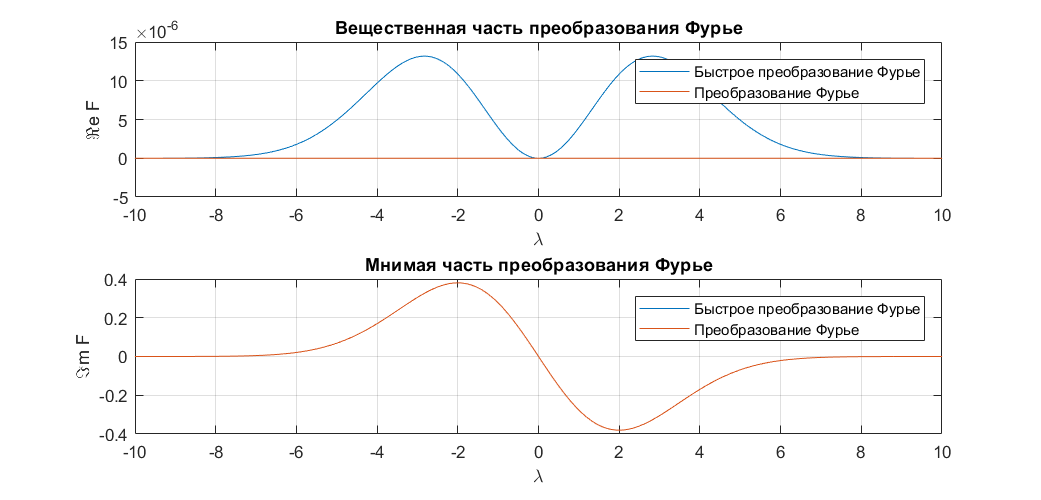
\includegraphics[width=\linewidth]{img/5.png}
                
                \begin{enumerate}
                    \item
                        Сравнивая данный график с предыдущим, мы понимаем, что существенных изменений нет. Отличие состоит лишь в том, что мы взяли другое окно. Отметим, что оно не является симметричным относительно начала координат. И здесь справедливы выводы, сделанные в предыдущем пункте.
                \end{enumerate}
            
            \item
                $\Delta t = 1$, $[a;\; b] = [-20;\; 50]$, $[c;\;d] = [-7;\;7]$.
                
                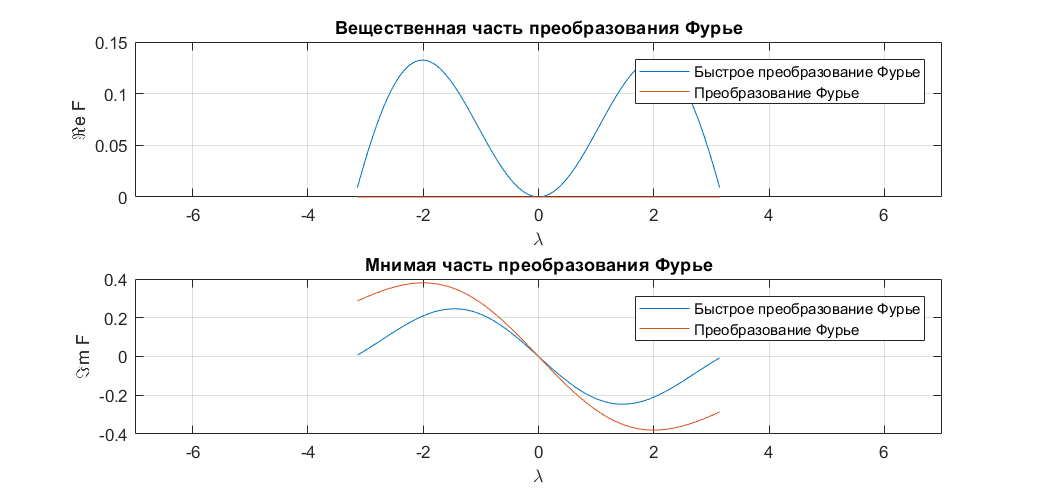
\includegraphics[width=\linewidth]{img/6.png}
                
                \begin{enumerate}
                    \item
                        Вещественная часть преобразования Фурье по-прежнему равна нулю, поэтому сдвиг ничего не изменит.
                    \item
                        Что касается мнимой части,то здесь наблюдается эффект наложения спектра (т.е. сумма исходного аналитического преобразования Фурье и сдвинутых аналитических преобразований Фурье равна численному преобразованию Фурье в каждой точке $\lambda$ из отрезка$\left[-\frac{\pi}{\Delta t}; \frac{\pi} {\Delta t} \right]$). При этом численное преобразование Фурье не совпадает с аналитическим.
                        
                        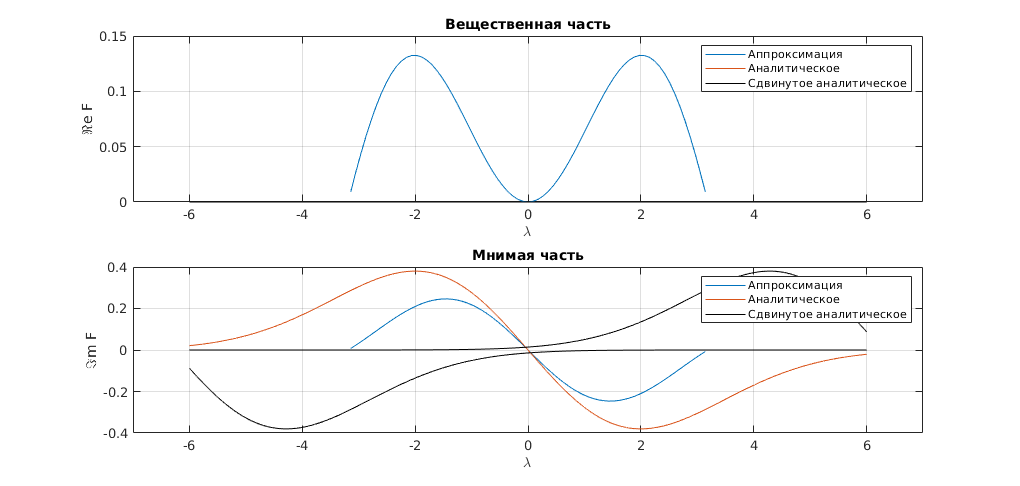
\includegraphics[width=\linewidth]{img/shifted.png}

                        Данное явление обусловлено нарушением соотношения $$\Delta t \leq \frac{\pi} {\Lambda},$$ где $\Delta t$ — шаг дискретизации, а $\Lambda > 0$ $(|\lambda| < \Lambda)$ — промежуток, где нужно устранить наложение спектра. В данном случае эффект наложения спектра можно устранить, т.к. функция $F_1(\lambda) \longrightarrow 0$, при $|\lambda|\longrightarrow +\infty$. И чтобы его устранить, нужно увеличить окно и уменьшить шаг дискретизации $\Delta t$.
                \end{enumerate}
        \end{enumerate}
    \subsection{Третья функция}
        Рассмотрим функцию        
        $$
            f_3(t)=\frac{2}{1+3t^6}.
        $$
        \begin{enumerate}
            \item
                $\Delta t = 10^{-4}$, $[a;\; b] = [-100;\; 100]$, $[c;\;d] = [-10;\;10]$
                
                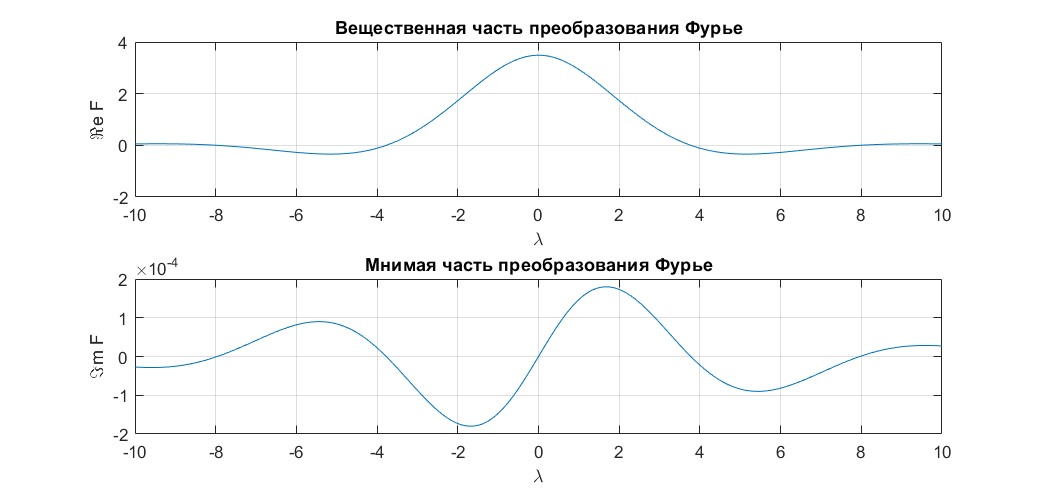
\includegraphics[width=\linewidth]{img/7.png}
            \item
                $\Delta t = 10^{-1}$, $[a;\; b] = [-100;\; 100]$, $[c;\;d] = [-10;\;10]$
                
                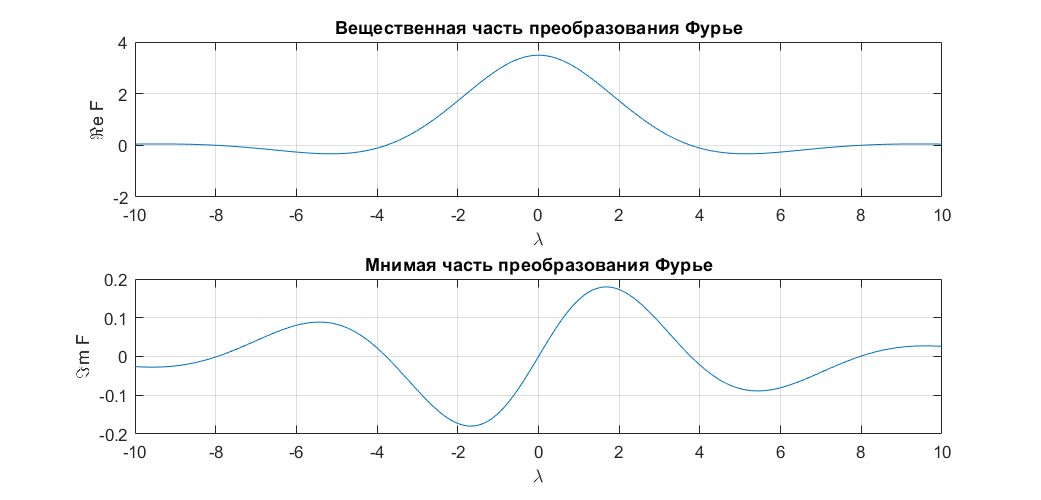
\includegraphics[width=\linewidth]{img/8.png}
        \end{enumerate}
        
        Из приведённых графиков следует:
        \begin{itemize}
            \item
                Мнимая часть преобразования Фурье равна нулю. Это следует из того, что если мы будем стремить шаг дискретизации к нулю, то максимальное значение преобразования Фурье тоже будет стремиться к нулю.
            \item
                Преобразование Фурье данной функции является непрерывным.
        \end{itemize}
    \subsection{Четвёртая функция}
        Рассмотрим функцию:
        $$
            f_4(t)=e^{-5|t|} \cdot ln(3+t^4).        
        $$
        \begin{enumerate}
            \item
                $\Delta t = 10^{-2}$, $[a;\; b] = [-100;\; 100]$, $[c;\;d] = [-15;\;15]$
                
                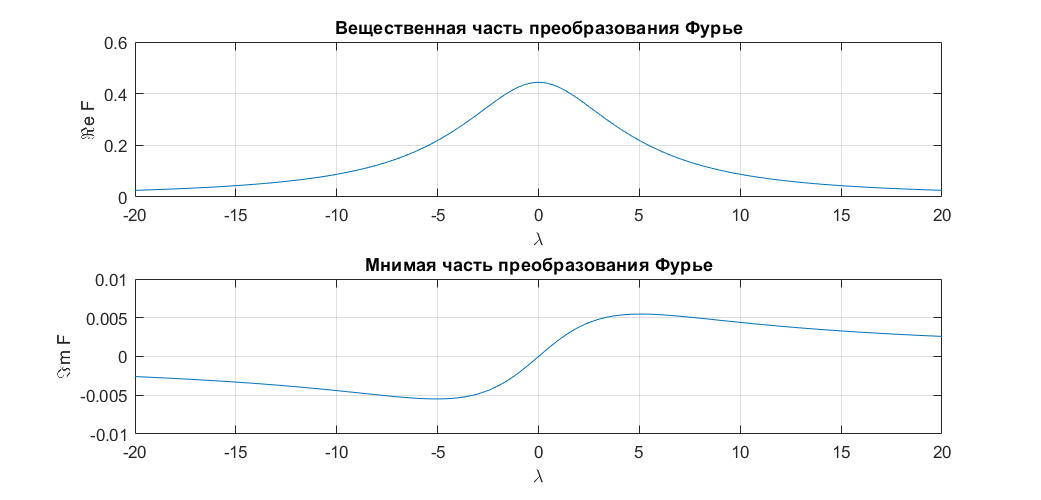
\includegraphics[width=\linewidth]{img/9.png}
            \item
                $\Delta t = 10^{-4}$, $[a;\; b] = [-20;\; 300]$, $[c;\;d] = [-20;\;20]$
                
                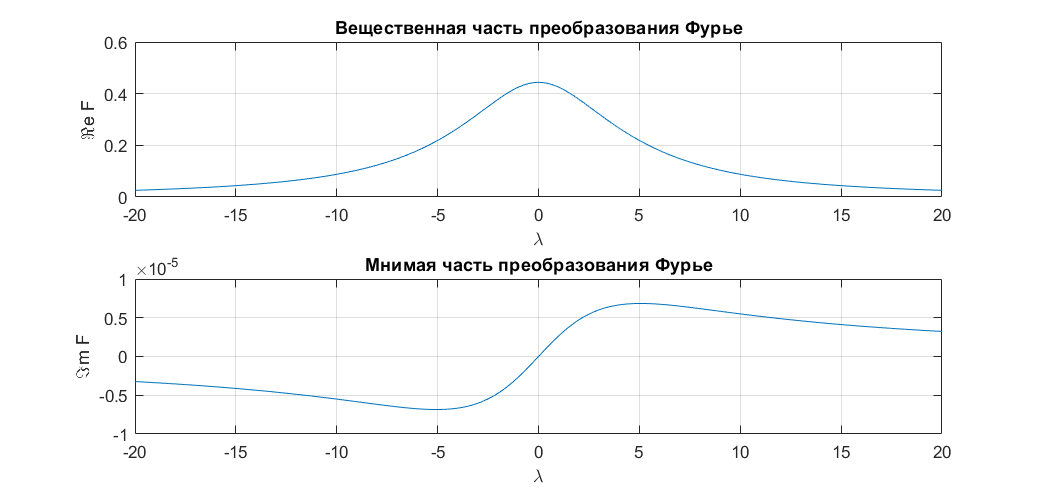
\includegraphics[width=\linewidth]{img/10.png}
        \end{enumerate}
        
        Сравнив два графика, видим:
        \begin{itemize}
            \item
                Существенных изменений не произошло, несмотря на то, что были изменены все параметры. Мнимая часть равна нулю.
            \item
                Пробразование Фурье данной функции — непрерывно.
        \end{itemize}
\clearpage
\section{Заключение}
    В ходе выполнения работы:
    \begin{enumerate}
        \item
            Были вычисленны преобразования Фурье двух функций. Произведено сравнение аналитических преобразований Фурье с их аппроксимациями.
        \item
            Были изучены различные явления, возникающие в ходе аппроксимации преобразования Фурье: рябь, вызванная разрывностью преобразования, рябь, вызванная асимметричностью окна, и эффект наложения хвостов.
        \item
            При использованиибыстрого преобразования Фурье, в силу его дискретной природы, могут быть получены неточные результаты. При правильном же подборе параметров результат будет приближаться к аналитическому решению, а в случае разрывного преобразования --- предсказуемо отклоняться от него.
    \end{enumerate}
\begin{thebibliography}{99}
	\bibitem{merlini} И.~В.~Рублёв. Лекции по преобразованиям Лапласа-Фурье. 2018
	\bibitem{ilinpoznyak}Ильин,~В.~А. Основы математического анализа. В 2 ч. Ч.2. 5-е изд. / В.~А.~Ильин, Э.~Г.~Позняк. --- М.: Физматлит, 2009.
	\bibitem{stolik} А.~В.~Столяров. Сверстай диплом красиво: \LaTeX за три дня. М.: МАКС Пресс, 2010. (\url{http://www.stolyarov.info/books/pdf/latex3days.pdf})

\end{thebibliography}
    
\end{document}
